%tapered_extension
Moreover, there are other optional designs for tapered waveguide can be involved to improve the Fiber-to-Chip coupling.  
In the other simulations of coupling between TLF and tapered waveguide there is another interesting result. If the taper is made from a proper material different from both guide and substrate, a more efficient coupling can be achieved in compare with our previous designs. For example, for a taper chosen for $n=2.0$, $d_{1}=2\mu$m and $L_{taper}=5.5\mu$m the coupling efficiency reaches $|S_{21}|=63\%$.  Because this design is not easy for fabrication,no more attention will be paid on it in this section.   
\begin{figure}[!ht]
\centering
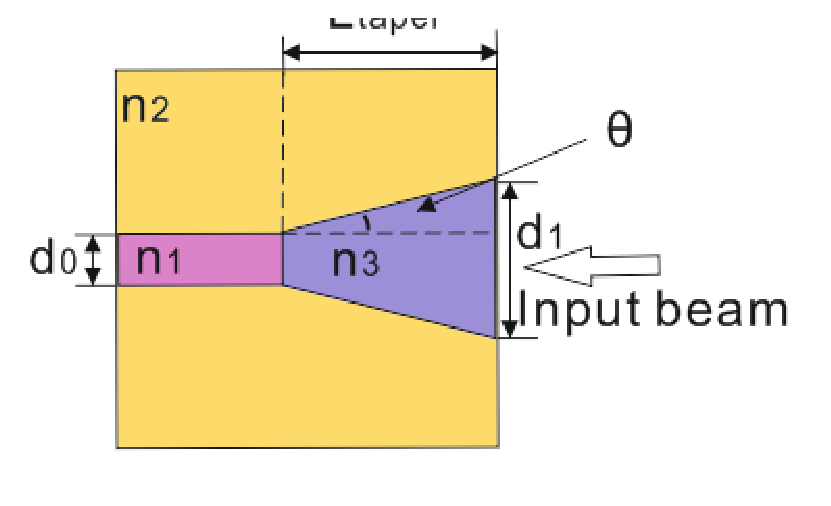
\includegraphics[width=0.7\textwidth]{bilder/tapered_waveguide_others}
\caption{Schema of a taperd waveguide combined with two different materials.}
\label{fig:tapered_waveguide_others}
\end{figure}

\cite{tapered_plasmonic_waveguides} mentions a tapered plasmonic waveguide, which is composed of a taper shape metal film on the dielectric substrate.  Under surface Plasmon polariton (SPP) wave 
\begin{figure}[!ht]
\centering
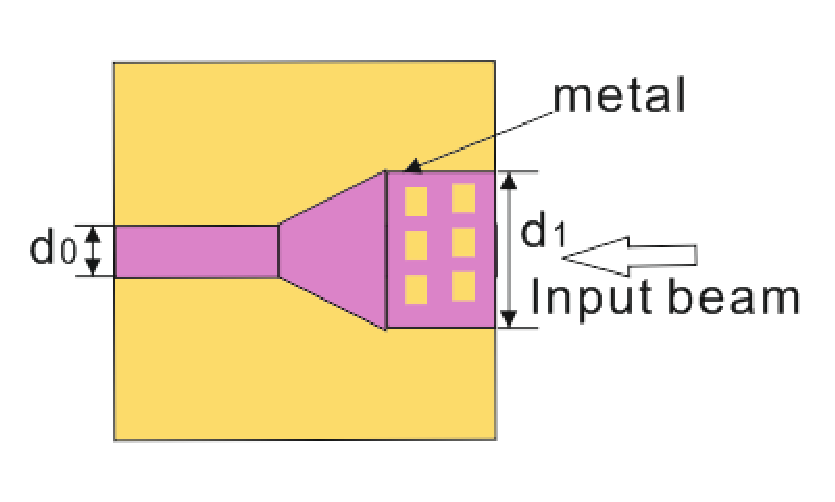
\includegraphics[width=0.7\textwidth]{bilder/tapered_waveguide_plasmonic}
\caption{Schema of a taperd plasmonic waveguide.}
\label{fig:tapered_waveguide_plasmonic}
\end{figure}


\cite{fiber_to_chip_grating_waveguides} provide a inversely tapered waveguide with gratings.
\begin{figure}[!ht]
\centering
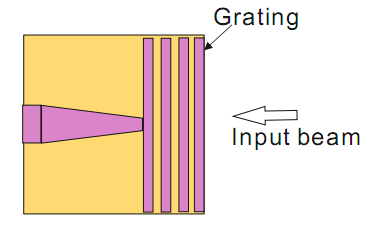
\includegraphics[width=0.7\textwidth]{bilder/tapered_waveguide_grating}
\caption{Schema of a taperd waveguide with grating.}
\label{fig:tapered_waveguide_grating}
\end{figure}
